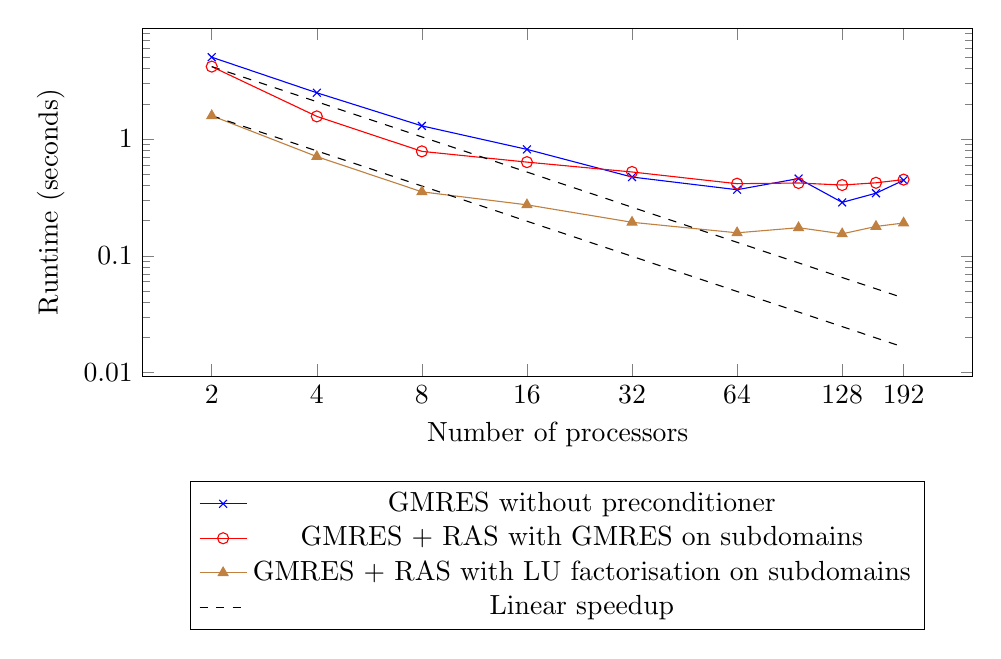
\begin{tikzpicture}
 \begin{axis}[
  height=6cm,
  width=\textwidth,
  xlabel=Number of processors,
  xtick={2, 4, 8, 16, 32, 64, 128, 192},
  xmode=log,
  ymode=log,
  log ticks with fixed point,
  ylabel=Runtime (seconds),
  legend style={
   at={(0.5, -0.3)},
   anchor=north
  }]
   \addplot[color=blue, mark=x] coordinates {
    (2, 5.019035956)
    (4, 2.489311578)
    (8, 1.295918689)
    (16, 0.8153684889)
    (32, 0.4725504889)
    (64, 0.3680468222)
    (96, 0.4586239333)
    (128, 0.2866520667)
    (160, 0.3435106444)
    (192, 0.4434605778)
   };
   \addlegendentry{GMRES without preconditioner}
   \addplot[color=red, mark=o] coordinates {
    (2, 4.171304311)
    (4, 1.562855289)
    (8, 0.78404696)
    (16, 0.6342229867)
    (32, 0.5220878222)
    (64, 0.4143123111)
    (96, 0.4201508889)
    (128, 0.4034540222)
    (160, 0.4217084444)
    (192, 0.4490838667)
   };
   \addlegendentry{GMRES + RAS with GMRES on subdomains}
   \addplot[color=brown, mark=triangle*] coordinates {
    (2, 1.583247378)
    (4, 0.7071820222)
    (8, 0.3530209556)
    (16, 0.2730702667)
    (32, 0.193635)
    (64, 0.1572552667)
    (96, 0.1740185111)
    (128, 0.1541527111)
    (160, 0.1782941778)
    (192, 0.1908772667)
   };
   \addlegendentry{GMRES + RAS with LU factorisation on subdomains}
   \addplot[color=black, domain=2:192, dashed] expression {
    4.171304311*2/x};
   \addlegendentry{Linear speedup}
   \addplot[color=black, domain=2:192, dashed] expression {
    1.583247378*2/x};
 \end{axis}
\end{tikzpicture}
